\documentclass[10pt,twocolumn,letterpaper]{article}

\usepackage{wacv}
\usepackage{times}
\usepackage{epsfig}
\usepackage{graphicx}
\usepackage{placeins}
\usepackage{amsmath}
\usepackage{amssymb}
\usepackage{subcaption}
\usepackage{threeparttablex,multirow,booktabs} % For formal tables
\usepackage[noend]{algpseudocode}
\usepackage[ruled,vlined,boxed,linesnumbered]{algorithm2e}
\usepackage{mathrsfs}
\usepackage{bm}
\usepackage[colorlinks=black,linkcolor=black,anchorcolor=black,citecolor=black]{hyperref}
\usepackage{caption}

% Include other packages here, before hyperref.

% If you comment hyperref and then uncomment it, you should delete
% egpaper.aux before re-running latex.  (Or just hit 'q' on the first latex
% run, let it finish, and you should be clear).
%\usepackage[pagebackref=true,breaklinks=true,letterpaper=true,colorlinks,bookmarks=false]{hyperref}

\wacvfinalcopy % *** Uncomment this line for the final submission

\def\wacvPaperID{477} % *** Enter the wacv Paper ID here
\def\httilde{\mbox{\tt\raisebox{-.5ex}{\symbol{126}}}}

% Pages are numbered in submission mode, and unnumbered in camera-ready
\ifwacvfinal\pagestyle{empty}\fi
\setcounter{page}{1}
%\begin{document}

%%%%%%%%% TITLE
\title{\textsc{Line Artist}: A Multi-style Sketch to Painting Synthesis Scheme}

% Authors at the same institution
%\author{First Author \hspace{2cm} Second Author \\
%Institution1\\
%{\tt\small firstauthor@i1.org}
%}
% Authors at different institutions
\author{Siqi Liu, Jinning Li \\
Shanghai Jiao Tong University\\
{\tt\small magi-yunan, lijinning@sjtu.edu.cn}
\and
Mengyao Cao \\
Shanghai Jiao Tong University\\
{\tt\small cmy\_0622@sjtu.edu.cn}
}
\begin{document}
\twocolumn[{%
\renewcommand\twocolumn[1][]{#1}%
\maketitle
\begin{center}
    \centering
    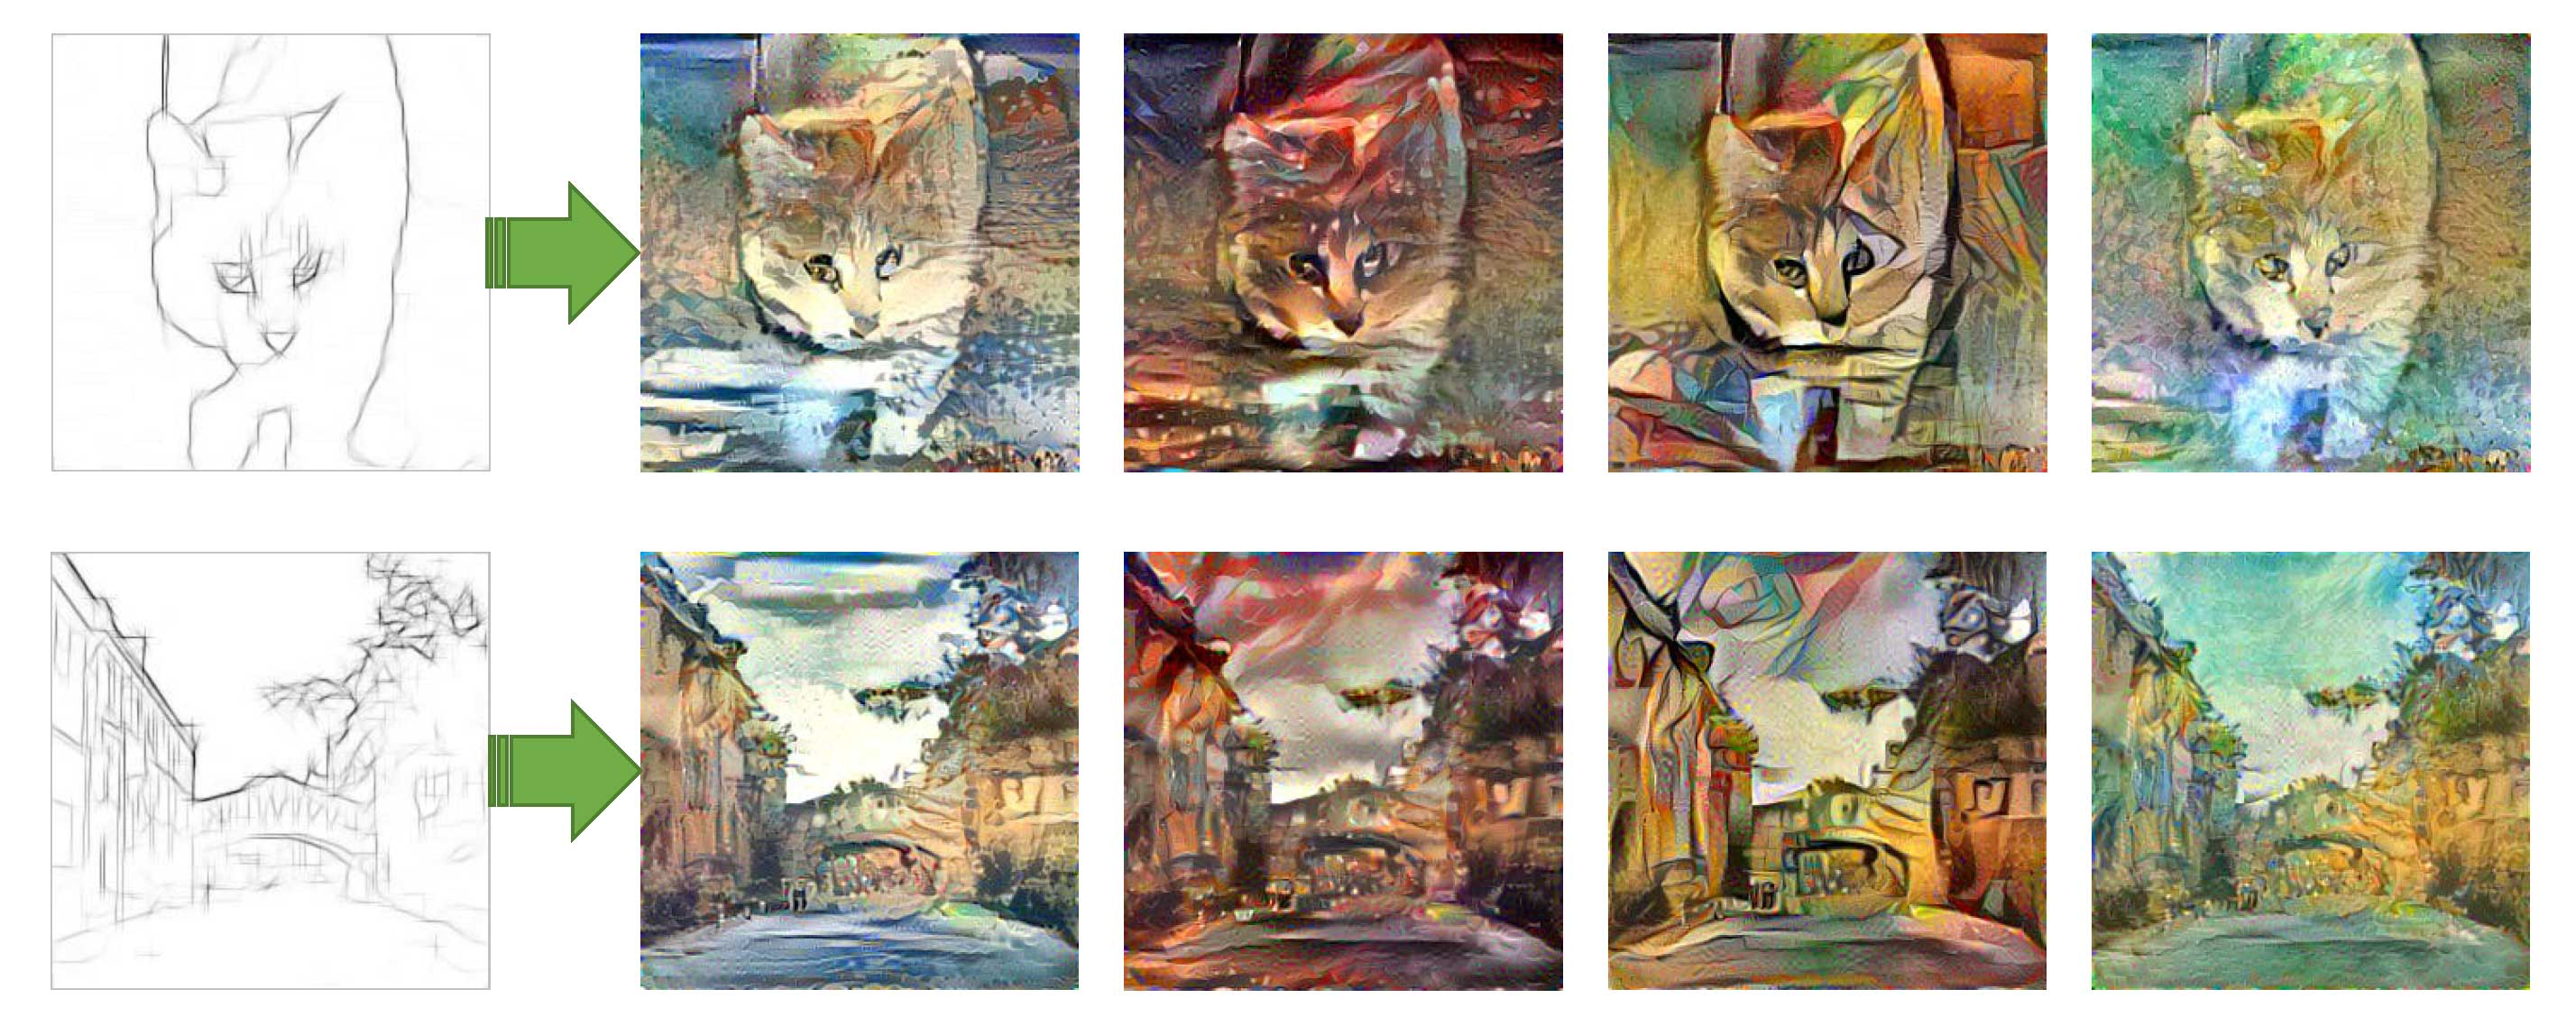
\includegraphics[width= 1.0\textwidth]{firstPage.jpg}
    \captionof{figure}{Stylizd images synthesized by \textsc{Line Artist} with sktch images}
    \label{fig::heading}
\end{center}%
}]

%\maketitle
\ifwacvfinal\thispagestyle{empty}\fi

%%%%%%%%% ABSTRACT
%\begin{figure*}[!htb]
%  %
%  \begin{subfigure}[b]{0.18\textwidth}
%    \includegraphics[width=\textwidth]{figure/catheading/sketch.png}
%    % \caption{Sketch}
%    % \label{fig::goldreal}
%  \end{subfigure}
%  \hspace{20px}
%  \begin{subfigure}[b]{0.18\textwidth}
%    \includegraphics[width=\textwidth]{figure/catheading/yys.jpg}
%    % \caption{Result of Gatys et al.}
%    % \label{fig::goldgatys}
%  \end{subfigure}
%  %
%  \begin{subfigure}[b]{0.18\textwidth}
%    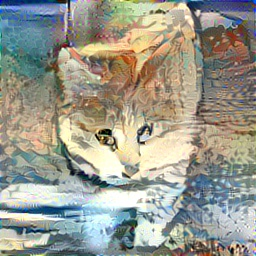
\includegraphics[width=\textwidth]{figure/catheading/fsh.jpg}
%    % \caption{Result of Ours}
%    % \label{fig::goldours}
%  \end{subfigure}
%  %
%  \begin{subfigure}[b]{0.18\textwidth}
%    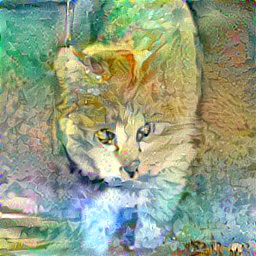
\includegraphics[width=\textwidth]{figure/catheading/fg.jpg}
%    % \caption{Result of Ours}
%    % \label{fig::goldours}
%  \end{subfigure}
%  %
%  \begin{subfigure}[b]{0.18\textwidth}
%    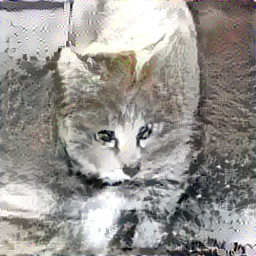
\includegraphics[width=\textwidth]{figure/catheading/chinese.jpg}
%    % \caption{Result of Ours}
%    % \label{fig::goldours}
%  \end{subfigure}
%  %
%  \begin{subfigure}[b]{0.18\textwidth}
%    \includegraphics[width=\textwidth]{figure/building/sketch.png}
%    \caption{Sketch}
%    % \label{fig::goldreal}
%  \end{subfigure}
%  \hspace{20px}
%  %
%  \begin{subfigure}[b]{0.18\textwidth}
%    \includegraphics[width=\textwidth]{figure/building/yys.png}
%    \caption{Onmyoji}
%    % \label{fig::goldgatys}
%  \end{subfigure}
%  %
%  \begin{subfigure}[b]{0.18\textwidth}
%    \includegraphics[width=\textwidth]{figure/building/fsh.png}
%    \caption{Ukiyo-e}
%    % \label{fig::goldours}
%  \end{subfigure}
%  %
%  \begin{subfigure}[b]{0.18\textwidth}
%    \includegraphics[width=\textwidth]{figure/building/fg.png}
%    \caption{Van Gogh}
%    % \label{fig::goldours}
%  \end{subfigure}
%  %
%  \begin{subfigure}[b]{0.18\textwidth}
%    \includegraphics[width=\textwidth]{figure/building/chinese.png}
%    \caption{Chinese painting}
%    % \label{fig::goldours}
%  \end{subfigure}
%  \caption{Result of \textsc{Line Artist}: translate the sketch images into paintings with different artistic styles}
%  % \label{fig::goldbridge}
%\end{figure*}%

\begin{abstract}
Drawing a beautiful painting is a dream of many people since childhood. In this paper, we propose a novel scheme \textsc{Line Artist} to synthesize artistic style paintings with freehand sketch images, leveraging the power of deep learning and advanced algorithm.

Our scheme includes three models. The \textit{Sketch Image Extraction} (SIE) model is applied to generate the training data. It includes smoothing reality images and pencil sketch extraction. The \textit{Detailed Image Synthesis} (DIS) model trains a conditional adversarial net to generate reality detailed information. The \textit{Adaptively Weighted Artistic Style Transfer} (AWAST) model is capable to combine multiple style image with content via VGG19 network and PageRank algorithm. The appealing stylized images are then generated by optimization iterations.

Experiments are operated on the Kaggle Cats dataset and The Oxford Buildings Dataset. Our synthesis results are artistic, beautiful and steadier. Real sketch tests prove that our scheme performs very well on reality environments. With different artist styles, our scheme can generate paintings of various styles. With our scheme, everyone can draw a beautiful picture only by drawing a sketch and then feeding it into our system.
\begin{figure*}[htb]
  %	\vspace{-1mm}
  \centering
  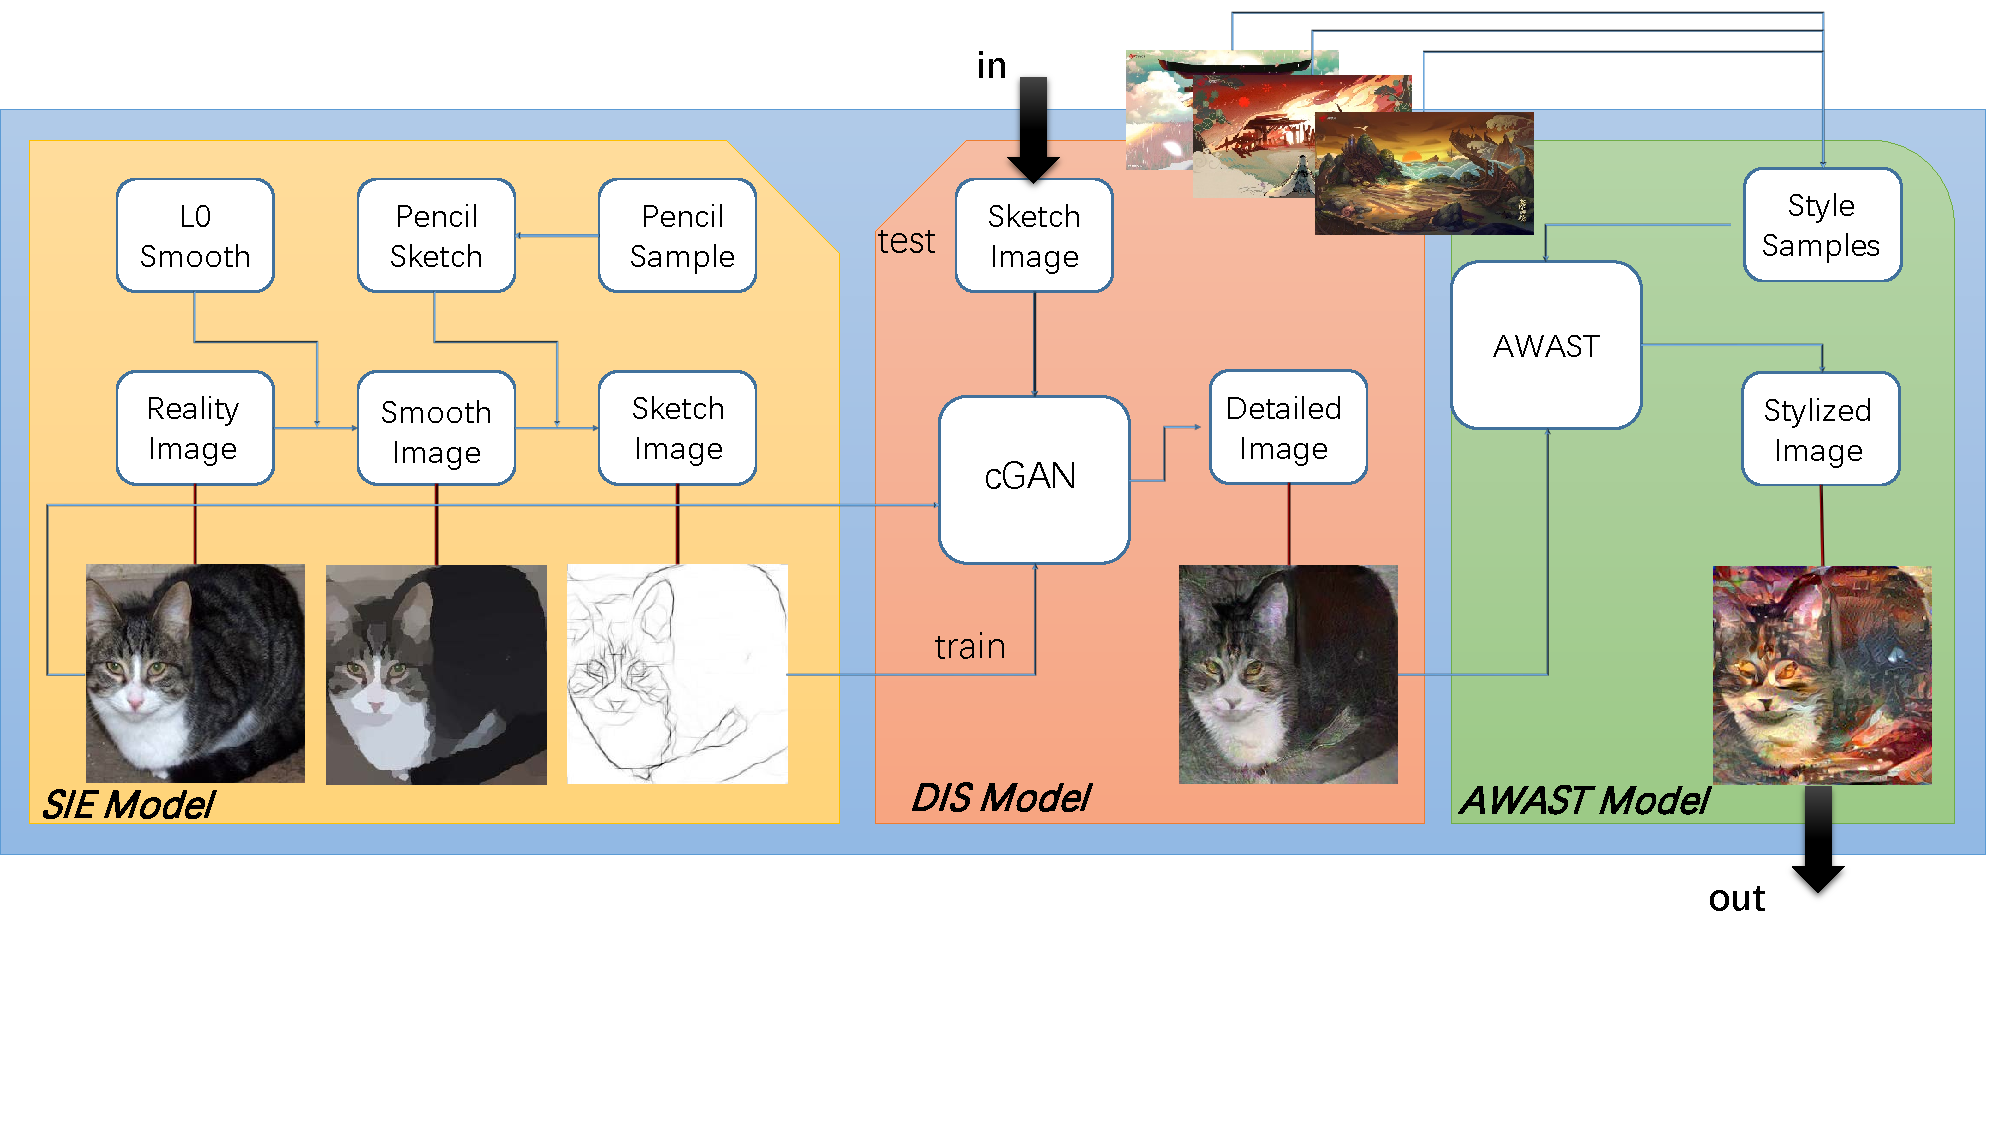
\includegraphics[width = 1\linewidth]{figure/overFlow2.pdf}
  %	\vspace{-9mm}
  \caption{Overview of \textsc{Line Artist}}
  \label{fig::overallFlow}
  %	\vspace{-4mm}
\end{figure*}
\end{abstract}
%%%%%%%%% BODY TEXT
\section{Introduction}
Deep learning has been applied to many scientific and engineering fields. However, researches on artist production are still limited. In our world, there are many people who want to paint beautiful paintings but feel depressed at not good at coloring. So we are considering creating a method using machine learning to help make some people's dream come true.

In this paper, we propose a new scheme, \textsc{Line Artist}, to paint like a well-known painter. The only thing need to be done is to draw some sketch lines. Then, \textsc{Line Artist} will drawing a meaningful and elegant painting for you like images in Fig.\ref{fig::heading}. Everybody can become a skilful painter!

Much work has been done to transform a real-world image into a stylized one. However, in our work, we aim at generating an artist style painting from a freehand sketch. Our scheme is able to extract the information from the sketch draft, generate a detailed image with new information using GAN. Then, we apply an Adaptively Weighted Artistic Style Transfer~\cite{gatys2015neural} algorithm based on VGG19~\cite{simonyan2014very} convolutional neural network and PageRank algorithm to transform our synthesized detailed image into a stylized one.

In order to train a supervised system receiving a sketch image and generating a more informative detailed image in Section~\ref{subsec::DIS}, a corresponding training dataset is needed. However, there is no such dataset published and building a new one will cost a large scale of time and human resources. To solve this problem, we introduce the \textit{Sketch Image Extraction} (SIE) model to synthesize sketch-like images efficiently, whose color is yellow in Fig.\ref{fig::overallFlow}.

To extract the sketch more accurately, in the SIE model we employ the $L_0$-Smooth~\cite{xu2011image} algorithm to smooth the initial image in order to make the edges more distinct and wipe out the unnecessary veins. Then, we adapt the pencil drawing~\cite{lu2012combining} method to extract the sketch image from the smooth one. Through the SIE model, we obtain the dataset containing pairs of initial reality images and the corresponding sketch images.

To generate an informatively detailed image from a given sketch image, the \textit{Detailed Image Synthesis} (DIS) model is introduced whose color is orange in Fig.\ref{fig::overallFlow}. We use the dataset generated by the SIE model to train a system that receive the skech image extracted and output a detailed image by generating more information. In our test, by input the sketch draw by human, this system will also synthesize a good result. In this paper, we adopt the Pix2Pix~\cite{isola2016image} algorithm to the do the synthesis operation.

Finally, the \textit{Adaptively Weighted Artistic Style Transfer} (AWAST) model, whose color is green in Fig.\ref{fig::overallFlow}. solves the problem of artist style transfer with multiple painting samples. Artist Style~\cite{gatys2015neural} is an efficient tool to combine two images with both low-level features and high-level features extracted from CNN. In this paper, we introduce the \textit{Adaptive Style Weight} (ASW) based on the feature similarity network and PageRank algorithm. Using ASW, multiple painting samples can be combined more naturally and beautiful. After these process, we obtain a colorful painting result only from a line sketch by an user.

The contributions of this paper are summarized as bellow:
\begin{itemize}
  \item A delicate sketch image synthesis scheme and two elaborate datasets containing pairs of reality images and corresponding sketch images.
  \item An efficient DIS model achieving more reality details from sketch images.
  \item A novel algorithm to adaptively combine multiple painting samples and synthesize appealing stylized images.
\end{itemize}

%-------------------------------------------------------------------------
\section{Related Works}
\paragraph{\textbf{Sketch Extraction}}
Many researches~\cite{gonzalez2016improved, kumar2017fractional, gao2010improved}focus on the edge extraction based on algebraic algorithm like sobel operator and fuzzy mathematics. These traditional edge extraction methods are good substitutions of sketch and usually run fast. However, the trends and continuity of extracted edges are not as natural as man-made ones. In~\cite{Dollar_2013_ICCV}, the author propose a random forest based method to detect edge. In the reference~\cite{xie15hed}, the author propose a CNN-based edge detection algorithm, which performs better than the traditional ones. In the paper~\cite{wei2017road}, the author propose a RSRCNN to extract roads from aerial images, which can also be applied to the sketch extraction. However, the CNN-based methods are highly relied on the training datasets and cost a lot to train a network. In~\cite{zhang2015face} the author propose a face sketch synthesise scheme based on greedy search, this technique can synthesis sketch for other objects. However, its effect is more like a grey transfer than sketch extraction.
In~\cite{zhang2015segment, xu2011image}, efficient methods of image smoothing are proposed based on wave pattern, which is helpful preprocessing for extraction.
In~\cite{lu2012combining}, Lu propose a fast scheme to synthesize pencil drawing sketch image. The result is very appealing.

\textbf{Detail Synthesis}
In~\cite{sangkloy2016scribbler, isola2016image, odena2016conditional}, methods extended from GAN are used to synthesize detailed images with more information from given materials. These models are usually easier to train while the result are more fuzzy to some extent. Chen proposed an end-to-end cascaded refinement networks in~\cite{chen2017photographic} to synthesize large-size reality image from semantic layouts, whose result has a high resolution and accuracy. But this method is highly dependent on training datasets.
In~\cite{ho2016laplacian}, the author propose an image synthesis model based on Laplacian pyramid, which has a lower computation complexity.
In~\cite{pathak2016context}, Context Encoders,  a GAN based model, is promoted to generate more information from the surroundings, in which artist style could be applied.

\textbf{Style Transfer}
Most researches about style transfer focus on the combination of content and single style. In~\cite{huang2015synthesis}, initial content is transformed into oil style by pixel-level analysis. Gatys et al.~\cite{gatys2015neural} proposed a style transfer scheme based on CNN whose results are quite appealing. The model in~\cite{li2016combining} combines markov random fields with~\cite{gatys2015neural}.
In~\cite{ulyanov2016texture}, a faster feed-forward style image synthesis network is proposed.
Texture synthesis is used to transfer image style in \cite{elad2017style}. In this paper, multiple styles are combined together to synthesize appealing results with PageRank~\cite{page1999pagerank} in undirected graph~\cite{mihalcea2004textrank}.

%symbol table
% $\bm{\hat{s}}$ freehand sketch image
% $\bm{p_s}$ synthesized painting
% reality image $\bm{r}$
% $l_0(\bm{x})$ L0-Smooth
% edge extraction $ext(\bm{x})$
% contributive edge image $\bm{c}$
% $g(\cdot)$ DCGAN-AS
% sketch samples $\bm{S_{sample}}$
% sketch-like edge image $\bm{\bar{s}}$
%

\section{Formulation}
Our scheme includes three models: the \textit{Sketch Image Extraction} (SIE) model, the \textit{Detailed Image Synthesis} (DIS) model ,and the \textit{Adaptively Weighted Artistic Style Transfer} (AWAST) model.The overall goal of our scheme is to receive a freehand sketch image $\bm{\hat{s}}$ and then generate a synthesized painting $\bm{p_s}$ with artist style. The overview of our scheme is shown in Fig.\ref{fig::overallFlow}.

% Then, pairs of reality images and contributive edge image, which is denoted by $\bm{Pair_{R,C}}=\{(\bm{r},\bm{c})|\bm{r}\in \bm{R}, \bm{c}\in \bm{C}, \bm{c} = l_0\circ e(\bm{r})\}$ and the set of sketching samples $\bm{S_{sample}}$ is converted to sketching-like edge image $\bm{\bar{s}}$ with the DCGAN-AS $d(\bm{r}, \bm{e}, \bm{S_{sample}})$:
\subsection{Sketch Image Extraction Model}\label{subsec::SIE}
The SIE model receives a reality image $\bm{r}$. After the L0-Smooth process denoted by $l_0(\bm{x})$, $\bm{r}$ is transformed to the smooth image $\bm{m}$. Then, the sketch extraction algorithm $ext(\bm{x})$ receives the smooth image and produce the sketch image $s$.

\begin{equation*}
  \bm{S} = ext(l_0(\bm{R})),
  \label{equ::contributiveimg}
\end{equation*}
where $\bm{S}$ and $\bm{R}$ are sets of $\bm{s}$ and $\bm{r}$.

Pairs of $\bm{r}$ and $\bm{s}$ is denoted by $\bm{[R,S]}=\{(\bm{r},\bm{s})|\bm{r}\in \bm{R}, \bm{s}\in \bm{S}\}$, where $\bm{S}$ is the set of $\bm{s}$.

\subsubsection{Image Smoothing}\label{subsubsec::smoothing}
Actually, if you take a photo $\bm{R}$ of something, say, a tree, there are complex edges. For example, the veins of the leaves. However, when we draw a picture, for most people, we cannot draw so well and so subtle. Instead, we only draw the overall edges. So our goal is to generate a painting from a simple sketch. The first task is to abandon the detail veins in $\bm{R}$.

Smoothing is a useful method to abandon the detail veins. When we smooth a picture, we erease those detailed edges. In this paper, we adopt $L_0$-Smooth~\cite{xu2011image}, an image smoothing algorithm via $L_0$ gradient minimization. For every pixel in $\bm{R}$, we denote the pixel map of the objective smooth image as $\bm{M}$, then the gradient in $\bm{M}_{i, j}$ is $\nabla \bm{M}_{i, j}=(\partial_x \bm{M}_{i, j}, \partial_y \bm{M}_{i, j})^T$. The gradient measure in $\bm{M}$ is:

\begin{equation}
cnt(\bm{M}) = \#\{(i, j)\mid |\partial_x \bm{M}_{i, j}| + |\partial_y \bm{M}_{i, j}| \neq 0\},
\label{equ::cnt}
\end{equation}
which counts the number of pixels in $\bm{M}$ where $|\partial_x \bm{M}_{i, j}| + |\partial_y \bm{M}_{i, j}| \neq 0$. The objection of the optimization process is:
\begin{equation}
  \min_{\bm{M}}\left\{\sum_{i, j}(\bm{M}_{i, j} - R_{i, j})^2 + \lambda \cdot cnt(\bm{M}) \right\}
  \label{equ::minM}
\end{equation}

In $L_0$-smooth algorithm, auxiliary variables $h_{i, j}$ and $v_{i, j}$ are introduced to calculate the minimization of Eqn.\ref{equ::minM}:

\begin{equation}
  \min_{\bm{M}, h, v}\left\{\sum_{i, j}(\bm{M}_{i, j} - R_{i, j})^2 + \lambda \cdot cnt(\bm{M}) + \epsilon(h, v)  \right\}
  \label{equ::minMhv}
\end{equation}
with $\epsilon = \beta((\partial_x\bm{M}_{i, j} - h_{i,j})^2 + (\partial_y\bm{M}_{i, j}-v_{i, j}))$. Then with $\bm{M}$ initialized by $\bm{R}$, the iteration will converge to the smooth image $\bm{M^*}$

\subsubsection{Canny Edge Extraction}\label{subsubsec::canny}
With the smooth image $\mathbf{M^*}$ extracted, we can extract the contributive edge image $\mathbf{C} = canny(M^*)$ by Canny operator. Here we adopt the Canny operator with Sobel method and double threshold. The result is shown in Fig.\ref{fig::ceeimg}. We can see that the overall shape of the tree is extracted without unexpected noise, which is much more like human sketch.
%Fig.\ref{fig::ceereality} is the original reality image $\mathbf{R}$. Fig.\ref{fig::ceesmooth} is the smooth image processed with iterations by Equ.\ref{equ::minMhv}, the veins of the cat's fur and the background. Fig.\ref{fig::ceeedge} shows the result after canny operator,

\begin{figure}[htb]
  %	\vspace{-1mm}
  \centering
  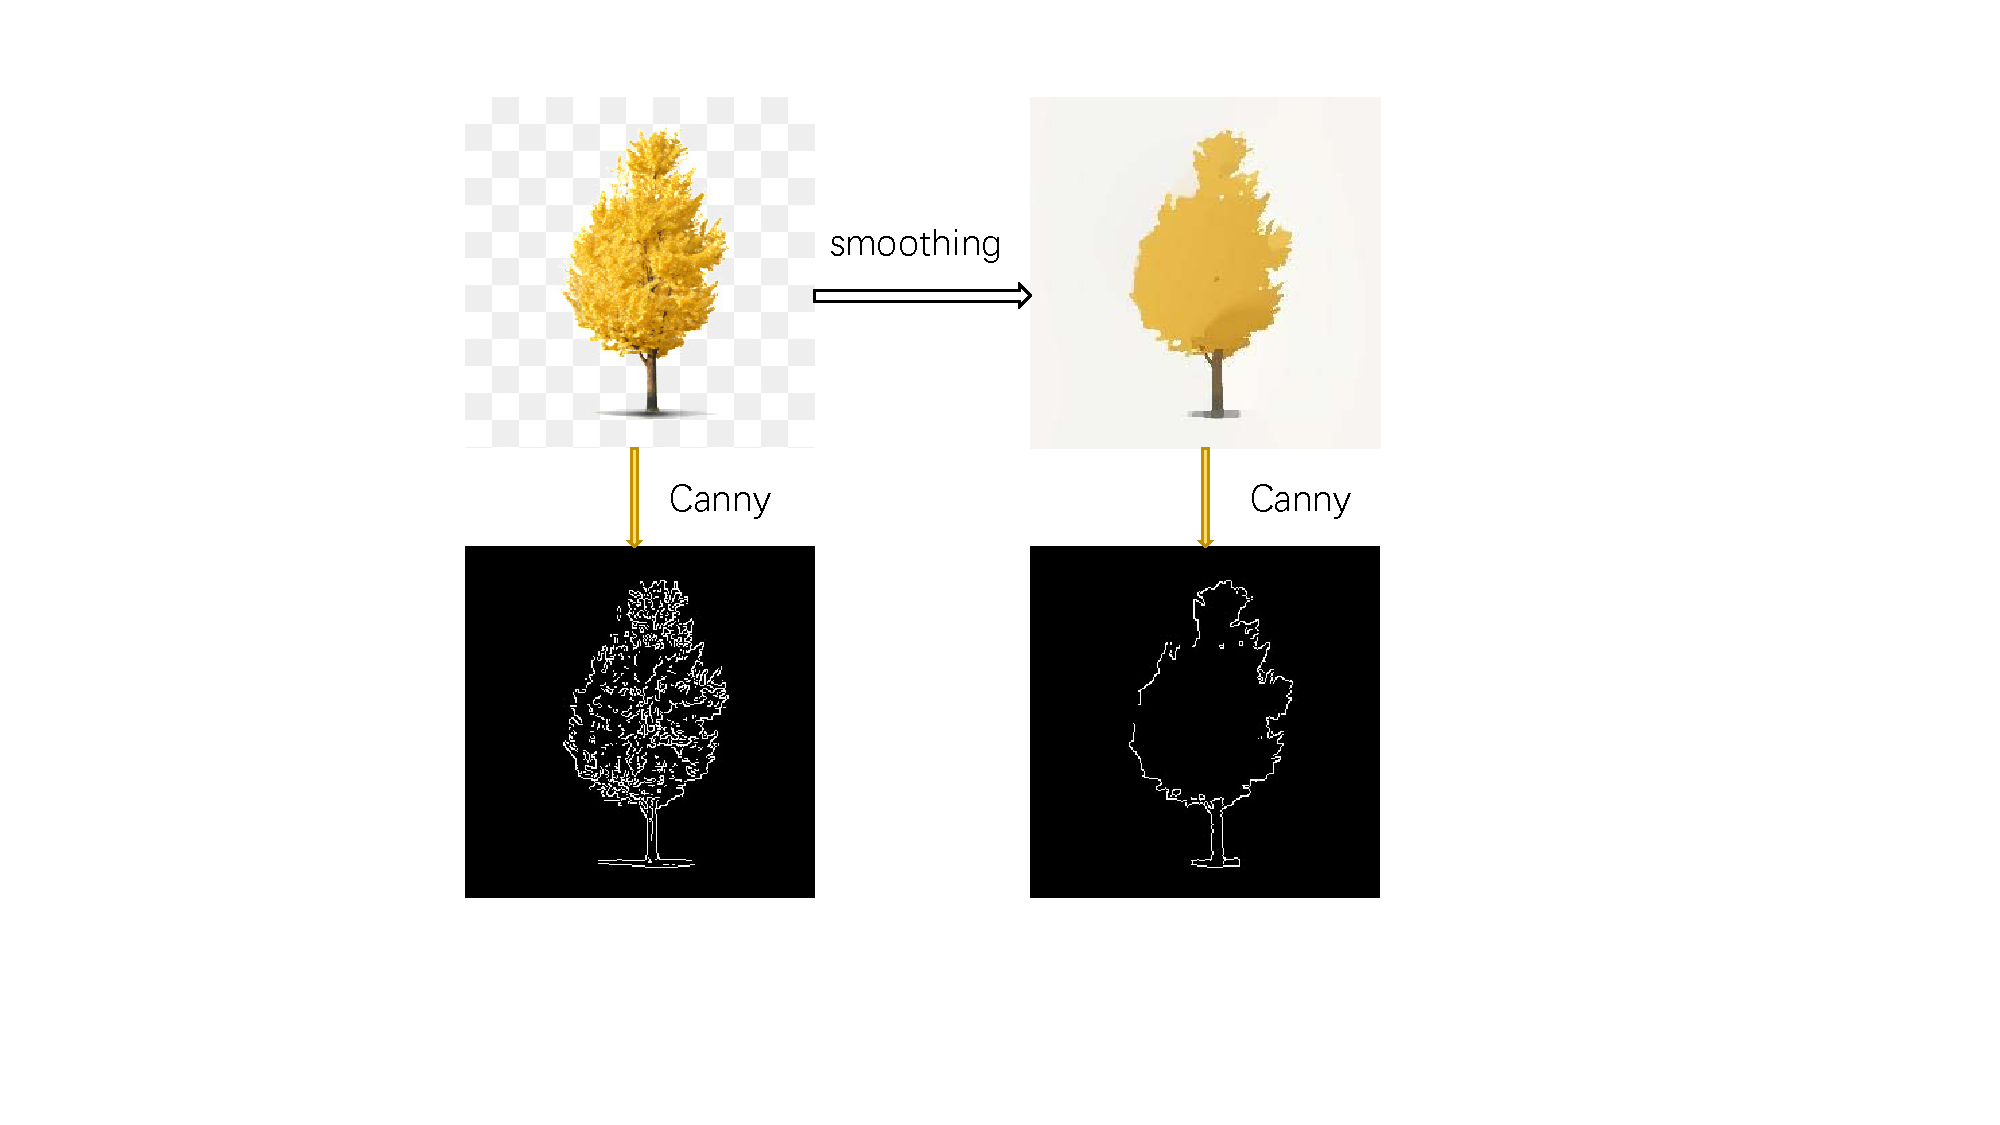
\includegraphics[width = 0.5\textwidth]{figure/originsmoothcanny.pdf}
  %	\vspace{-9mm}
  \caption{The different Canny result before and after smoothing. The upper left image is the origin image. The upper right is the smoothing one. The left lower is the edge of the origin image and the right lower is the edge of the smoothing one.}
  \label{fig::ceeimg}
  %	\vspace{-4mm}
\end{figure}

\subsubsection{Pencil Sketch Extraction}
Although a sketching-like image is already generated in Section~\ref{subsubsec::canny}, the line in the generated image $\mathbf{C}$ is not natural enough compared with real freehand sketching by humans. For most people, we cannot draw a line so long. There is always some break point.

In this way, the Canny generating picture is not what we want. To solve this problem, we use the the algorithm of producing pencil drawings from natural images~\cite{lu2012combining}. We mainly use the line drawing with strokes method, for we do not need pencil to draw the shadow.

In the line drawing from strokes method, there are some things we need notice. One thing is that artists always draw lines with breaks, not a long line without any break. Another thing is that there are always crosses at the junction of two lines.
Based on the two important thing, the method of drawing lines from strokes was born. When drawing strokes at a point, we determine the direction, length, and width in a pixel classification and link process based on a unified convolution framework.

\textbf{Classfication} We first transform the input image into grayscale version. Then compute the gradients of it, yielding magnitude
% \begin{center}
	\begin{equation}
	G = ((\partial_{x}I)^{2} + (\partial_{y}I)^{2})^{\frac{1}{2}}
	\end{equation}
% \end{center}
where I is the grayscale input, $\partial_{x}$ and $\partial_{y}$ are gradient operators in two directions, implemented by forward difference. Then we use local information to do the classification. We choose $8$(depending on the case, it may changed to $6$ or other value) directions, each is $45$ degrees apart and denote the line segment as $L_{i}$($i = 1, 2, ... , 8)$ representing the $8$ directions and the length of $L_{i}$ is $\frac{1}{30}$ of the height or width. So the responding map for a certain direction $i$ is
% \begin{center}
	\begin{equation}
	C_{i} = L_{i} * G
	\end{equation}
% \end{center}
where $*$ is the convolution operator. Finally, the classification is performed by choosing the maximum value among the response map in the $8$ directions. This step is written as
% \begin{center}
	\begin{equation}
		C_{i}(p) = \left\{
             \begin{array}{lr}
             G_{p}, &  if argmin_{i}[G_{i](p)} = i \\
             0, & otherwise
             \end{array}
\right.
\end{equation}
% \end{center}
where p indexes pixels and $C_{i}$ is the magnitude map for direction $i$.

\textbf{Line Shaping} We generate lines also by convolution given the map set $C_{i}$ and this is expressed like this
% \begin{center}
	\begin{equation}
	S^{'} = \sum_{i=1}^{8}(L_{i} \otimes C_{i})
	\end{equation}
% \end{center}

Convolution aggregates nearby pixels along direction $L_{i}$, which links edge pixels that are even not connected in the original gradient map.

Using these two method, we get freehand sketches, which are more like what ordinary people draw than using Canny.

% \begin{figure}
%   \begin{subfigure}[b]{0.15\textwidth}
%     \includegraphics[width=\textwidth]{figure/catline3.png}
%     \caption{Reality image}
%     \label{fig::ceereality}
%   \end{subfigure}
%   %
%   \begin{subfigure}[b]{0.15\textwidth}
%     \includegraphics[width=\textwidth]{figure/catline2.png}
%     \caption{Smooth image}
%     \label{fig::ceesmooth}
%   \end{subfigure}
%   %
%   \begin{subfigure}[b]{0.15\textwidth}
%     \includegraphics[width=\textwidth]{figure/catline1.png}
%     \caption{Extracted edge}
%     \label{fig::ceeedge}
%   \end{subfigure}
%   \caption{Images of CEE model}
%   \label{fig::ceeimg}
% \end{figure}

%
% \begin{figure}[htb]
%
% \begin{subfigure}[b]{0.4\linewidth}
% \centering
% \includegraphics[width=0.4\linewidth]{afig.png}
% \caption{The reality image}
% \end{subfigure}%
%
% \begin{subfigure}[b]{0.4\linewidth}
% \centering
% \includegraphics [width=0.4\linewidth]{afig.png}
% \caption {The extracted edge}
% \end{subfigure}%
%
% \caption{Example of sketching edge generating model}
% \end{figure}

\subsection{Detailed Image Synthesis Model}\label{subsec::DIS}
In DIS model, We adapt the \textit{conditional Generative Adversarial Networks} in~\cite{isola2016image}, which is denoted by $cGAN(\cdot)$. This architecture fits our work because cGAN runs fast and its precision is high enough for artistic synthesis. In the training process, $cGAN$ receive the pairs of reality and sketch images, $\bm{[\bar{S}, R]}$, generated in Section~\ref{subsec::SIE} to train the model. In the test process, the DIS model receives the real freehand sketch image $\bm{\hat{s}}$ and then generates a detailed informative image $\bm{d}$.

The loss function of CGAN is:
\begin{equation}
  \begin{split}
\mathcal{L}_{cGAN}(G, D) =& \mathbb{E}_{(s, r)\sim \bm{[\bar{S}, R]}}[logD(s, r)] +\\
&\mathbb{E}_{s\sim \bm{\bar{S}}, z}[log(1-D(s, G(s, z)))],
\end{split}
\end{equation}
where $G(\cdot)$ represents the generator, $D(\cdot)$ represents the discriminator.

In our work, $G$ is set to use the U-Net~\cite{ronneberger2015u}, which is similar to the Encoder-decoder architecture.

In order to make the results closer to reality, we adapt the objective cGAN with $L_1$ distance inspired by~\cite{pathak2016context}. By doing this, the generator is able to generate image more similar to the ground truth.

The compound objective is:
\begin{equation}
\mathcal{L} =  \mathcal{L}_{cGAN}(G, D) + \lambda \mathbb{E}_{(s, r)\sim \bm{[\bar{S}, R]}, z}[\|r-G(s, z)\|_1]
\end{equation}

Then, the objective generator by the optimization is:
\begin{equation}
 \bar{G} = \arg \min_G \max_D \mathcal{L}(G, D)
\end{equation}

with the objective $\bar{G}$ by training, we can generate the detailed image $d$ by $d = G(\hat{s})$.

%
%\begin{figure}[htb]
%
%\begin{subfigure}[b]{0.4\linewidth}
%\centering
%\includegraphics[width=0.4\linewidth]{afig.png}
%\caption{The edge image}
%\end{subfigure}%
%
%\begin{subfigure}[b]{0.4\linewidth}
%\centering
%\includegraphics [width=0.4\linewidth]{afig.png}
%\caption {The realized edge}
%\end{subfigure}%
%
%\caption{Example of Detailed Image Synthesis model}
%\end{figure}
%
%[text and formula]

\subsection{Adaptively Weighted Artistic Style Transfer} \label{subsec::AWAST}
The \textit{Adaptively Weighted Artistic Style Transfer} (AWAST) model recieves the detailed informative image $d$ synthesized in Section~\ref{subsec::DIS} and then given set of artistic style samples $A$. The features of the detailed image $d$ and the artistic samples $a\in A$ are extracted from the pretrained VGG19~\cite{simonyan2014very} net. An novel weight calculating algorithm based on PageRank is used to combine the features. Then, a random noise image $x$ was optimized to our objection image $g$, which combines both the low and high level features of $d$ and $A$.

The first step of AWAST is to feed $d$ and every $a$ into the pretrained VGG19 network inspired by the artistic style algorithm~\cite{gatys2015neural}. After this process, we obtain an activated feature map $\bm{F}_l$ on each convolutional layer$l$. Every activated feature map represents the different levels of features. In the beginning convolutional layer, more low-level information about color, pattern and details are extracted. And the high-level information like the distribution and shape is store in the latter convolutional layer.

We denote the set of activated feature maps for every artistic sample $a\in A$ as $\mathbb{F}_a$: $\mathbb{F}_a = \bigcup\{\bm{F}_{a,l}\}$. Similarly, we denote the extracted features of informative image $d$ as $\mathbb{F}_d = \bigcup\{\bm{F}_{d,l}\}$ and $\mathbb{F}_x = \bigcup\{\bm{F}_{x,l}\}$ for noise image $x$.

Our approach is optimizing $x$ by iteration $t$ to make sure it is similar to both $d$ and $a$ in $A$. So, we define the loss function of the optimization as:
\begin{equation}
\mathcal{L}(d, A, l, t) = \alpha \mathcal{L}_{1}(l, d, x_t) + \beta \sum_{l, a\in A}\bar{\omega}(l, a)\cdot \mathcal{L}_{2}(l, a, x_t),
\end{equation}\label{equ::overallloss}
where $\mathcal{L}_1(d, x_t)$ is the content loss between $d$ and $x_t$, $\mathcal{L}_2(a, x_t)$ is the style loss between $a$ and $x_t$. $\bar{\omega}(l, a)$ is the \textit{adaptive style weight} (ASW) of sample $a$ and layer $l$. $\alpha$ is the overall content weight and $\beta$ is the overall style weight.

The content loss $\mathcal{L}_1$ is defined as the squared error loss between $d$ and $x_t$: \begin{equation}
\mathcal{L}_1(l, d, x_t) = \frac{1}{2}\sum_{i,j}(F_{i, j, d}^{l}-F_{i, j, x_t}^{l}).
\end{equation}

The style loss is defined with the Eccentric covariance matrix(Gram) matrix $G^l$ in different layer $l$, $G^l_{i, j} = \sum_{k} F_{i, k}^l F_{j,k}^l$. Our optimization problem is converted to minimize the difference between the Gram matrix of $a$ and $x_t$. We define the style loss as
\begin{equation}
\mathcal{L}_2(l, a, x_t) = {\frac{1}{4n_lw_lh_l}\sum_{i,j}(G_{i, j, a}^{l} G_{i, j, x_t}^l)},
\end{equation}
where $\frac{1}{4n_lw_lh_l}$ is the normalization coefficient in order to make $\mathcal{L}_2$ compatible with $\mathcal{L}_1$

Recall that different $\bm{F}_{a, l}$ can represent different features, in another word, the painting skills of different artists. For example, in Pablo Picasso's painting, the high-level feature would contain more sharp, irregular geometry and lines while the low-lever feature would include deeper colors and smooth pattern. For Claude Monet's paiting, the features are almost opposite.

To make the artistic style painting synthesized from multiple artist painting samples $a\in A$ being more delicate and appealing, we introduce the \textit{adaptive style weight} (ASW) to balance the style futures from different samples and layers. Since multiple painting samples are input to our system, various styles and skills from different artists will pile up. In order to emphasize the most common used skills, factions, and color preference, etc. and weaking some minor and unimportant skills from these artists , we use ASW to balance the importance of them.

To calculate the ASW, we build a style similarity network and use the undirected PageRank algorithm~\cite{grolmusz2012note} to define the ASW.
We define the difference matrix $\Delta$ between different $F_{a, l}$ by the squared error:
\begin{equation}
\Delta_{p, q}^l = \frac{1}{2}\sum_{i, j}(F_{i, j, a_p}^l - F_{i, j, a_q}^l)^2.
\end{equation}
We define the similarity matrix $\Gamma$ as:
\begin{equation}
\Gamma_{p, q}^l = \frac{ \max_{i, j}\Delta_{i, j}^l } { \Delta^l_{p, q}}.
\end{equation}
The matrix $\Gamma^l$ is symmetric, full-rank and the diagnal element is zero. We build a fullly connected undirected graph according to $\Gamma^l$. The weight of edges in this graph is defined as: $\mu_{i, j}^l = \Gamma^l_{i, j} / \sum_{j}\Gamma^l_{i, j}$. The weight of nodes in this graph is denoted as $PR$, representing the importance of this node in the PageRank algorithm.

The iteration formulation of undirected PageRank is:
\begin{equation}
PR_t(p_i) = \frac{1-\theta}{N_s} + \frac{\theta}{N_s} \sum_{p_j\in E(p_i)}\mu_{p_i, p_j}PR_{t-1}(p_j),
\end{equation}\label{equ::pagerank}
where $p_i$ and $p_j$ are nodes in the graph. $\theta$ is the damping factor of PageRank algorithm. $N_s = |A|$ is the number of nodes. $E(p_i)$ is the set of nodes that connecting with $p_i$

Then, the matrix $\overline{PR}$ is obtained after the PageRank algorithm converged. Then, we define the ASW with a sigmoid mapping:
\begin{equation}
\omega(l, a) = (1 + exp( 2 - \frac{4(\overline{PR} - \min(\overline{PR}))} {\max(\overline{PR})- \min(\overline{PR})}))^{-1},
\end{equation}
By normalization, the ASW $\bar{\omega}(l, a) = \frac{1}{N_lN_s}\omega(l, a)$ is obtained.

Then, by minizing the overall loss in Eqn.\ref{equ::overallloss}, the random noise image $x$ will converge to the objection image $g$.
%\begin{figure}[htb]
%
%\begin{subfigure}[b]{0.4\linewidth}
%\centering
%\includegraphics[width=0.4\linewidth]{afig.png}
%\caption{before stylize}
%\end{subfigure}%
%
%\begin{subfigure}[b]{0.4\linewidth}
%\centering
%\includegraphics [width=0.4\linewidth]{afig.png}
%\caption {after stylize}
%\end{subfigure}%
%
%\caption{Example of Adaptively Weighted Artistic Style Transfer model}
%\end{figure}
%
%[text and formula]

\section{Experiments}
To evaluate the performance of our scheme, experiments of our scheme and baselines are set as below.

\textbf{Datasets:}\label{line::dataset}
For the SIE and the DIS model, we use the Cats dataset on Kaggle. However, we didn't use the whole dataset, we only choose $2620$ images in the dataset, extracting some images on which there are mainly human beings or something like that but not mainly cats. We also use the Oxford Buildings Dataset. We randomly choose $4202$ building images in this dataset.

For the AWAST model, we mainly choose style images from Google Image for the ink painting style, the Picasso style, the Van gogh style, the watercolor style and Ukiyo-e style. For the Onmyoji style, we choose images of a mobile game named Onmyoji of Netease Company in China.

\textbf{Environment:}
All the experiments are conducted on a PC device (Intel(R) Core(TM) i7-6900K 3.2GHz, 16GB memory, NVIDIA GeForce(R) GTX 1080 Ti) and are implemented in Python 3.6.2\footnote{All the code will be publicly available after the review process.}.

\subsection{Training}
Because our model is the combination of the three models mentioned above, we now describe the training process in three main steps corresponding to the three models.

In the SIE model, for smoothing, we set the parameters lamda to be $0.02$, kappa to be $1.2$. And for pencil sketching, we set the length of convolution line to be $7$, the width of the stroke to be $0.1$, the number of directions to be $10$ for the cat dataset. For the building dataset, we set the length of convolution line to be $7$, the width of the stroke to be $0.1$, the number of directions to be $10$. Because for some image in the two datasets, there are some pictures too complex for freehand drawing, we deleted these complex pictures.

The DIS model receives the training datasets from SIE, which are pairs of sketch images and the reality images. These images are resized to $256\times 256$ to accelerate our training speed. Then, we set the learning rate $lr = 0.0002$, the generator use the unet 256 network. The initialization of network is set to use xavier initializer. Both the input and output channels are set to be $3$.

The AWAST model receives the $256\times 256$-size images synthesized by the DIS model and the style image samples illustrated in Section~\ref{line::dataset}. The parameters $\alpha$ and $\beta$ in Eqn.\ref{equ::overallloss} are set as $8$ and $500$. The dumping factor of PageRank $\theta$ in Eqn.~\ref{equ::pagerank} is set to be $0.85$ and the convergent accuracy of PageRank is $0.0001$. The learning rate is $1$ and parameters $\beta_1$ and $\beta_2$ for Adam optimizer are $0.9$ and $0.999$. The iteration of optimization is set to be $2000$.

\begin{figure*}
  \centering
  %
  \begin{subfigure}[b]{0.18\textwidth}
    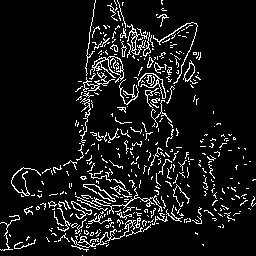
\includegraphics[width=\textwidth]{figure/baseline2/canny.jpg}
    \caption{Canny edge}
    \label{fig::base11}
  \end{subfigure}
  ~
  %
  \begin{subfigure}[b]{0.18\textwidth}
    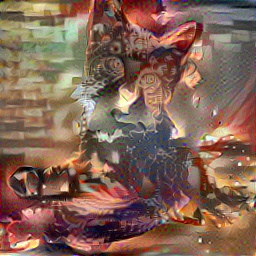
\includegraphics[width=\textwidth]{figure/baseline2/yys.jpg}
    \caption{Onmyoji}
    \label{fig::base12}
  \end{subfigure}
  %
  \begin{subfigure}[b]{0.18\textwidth}
    \includegraphics[width=\textwidth]{figure/baseline2/fsh.jpg}
    \caption{Ukiyo-e}
    \label{fig::base13}
  \end{subfigure}
  %
  \begin{subfigure}[b]{0.18\textwidth}
    \includegraphics[width=\textwidth]{figure/baseline2/fg.jpg}
    \caption{Van Gogh}
    \label{fig::base14}
  \end{subfigure}
  %
  \begin{subfigure}[b]{0.18\textwidth}
    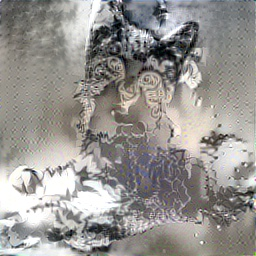
\includegraphics[width=\textwidth]{figure/baseline2/chinese.jpg}
    \caption{Chinese painting}
    \label{fig::base15}
  \end{subfigure}
  	% \vspace{-1mm}
  \caption{Baseline 1: Extract edge with canny algorithm and feed AWAST directly}
  \label{fig::cannyonly}
  %
  \begin{subfigure}[b]{0.18\textwidth}
    \includegraphics[width=\textwidth]{figure/baseline4/sketch.jpg}
    \caption{Sketch}
    \label{fig::base21}
  \end{subfigure}
  ~
  %
  \begin{subfigure}[b]{0.18\textwidth}
    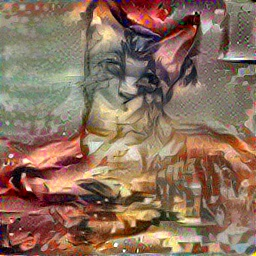
\includegraphics[width=\textwidth]{figure/baseline4/yys.jpg}
    \caption{Onmyoji}
    \label{fig::base22}
  \end{subfigure}
  %
  \begin{subfigure}[b]{0.18\textwidth}
    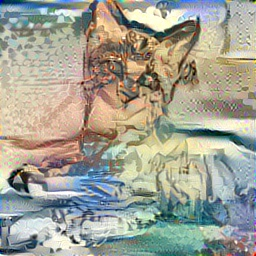
\includegraphics[width=\textwidth]{figure/baseline4/fsh.jpg}
    \caption{Ukiyo-e}
    \label{fig::base23}
  \end{subfigure}
  %
  \begin{subfigure}[b]{0.18\textwidth}
    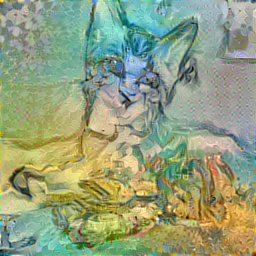
\includegraphics[width=\textwidth]{figure/baseline4/fg.jpg}
    \caption{Van Gogh}
    \label{fig::base24}
  \end{subfigure}
  %
  \begin{subfigure}[b]{0.18\textwidth}
    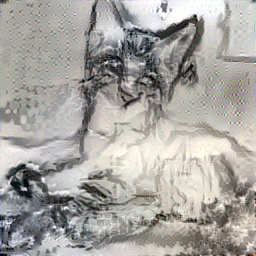
\includegraphics[width=\textwidth]{figure/baseline4/chinese.jpg}
    \caption{Chinese painting}
    \label{fig::base25}
  \end{subfigure}
  %	\vspace{-1mm}
  \caption{Baseline 2: Smoothing, extracting pencil sketh, and feeding the sketch to AWAST directly}
  \label{fig::sketchonly}
  %
  \begin{subfigure}[b]{0.18\textwidth}
    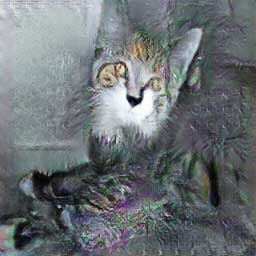
\includegraphics[width=\textwidth]{figure/baseline3/canny.jpg}
    \caption{Detailed image}
    \label{fig::base31}
  \end{subfigure}
  ~
  %
  \begin{subfigure}[b]{0.18\textwidth}
    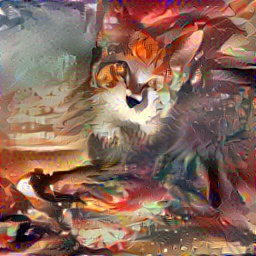
\includegraphics[width=\textwidth]{figure/baseline3/yys.jpg}
    \caption{Onmyoji}
    \label{fig::base32}
  \end{subfigure}
  %
  \begin{subfigure}[b]{0.18\textwidth}
    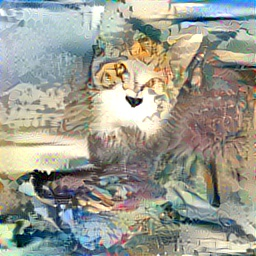
\includegraphics[width=\textwidth]{figure/baseline3/fsh.jpg}
    \caption{Ukiyo-e}
    \label{fig::base33}
  \end{subfigure}
  %
  \begin{subfigure}[b]{0.18\textwidth}
    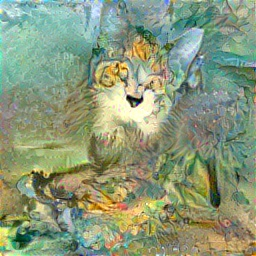
\includegraphics[width=\textwidth]{figure/baseline3/fg.jpg}
    \caption{Van Gogh}
    \label{fig::base34}
  \end{subfigure}
  %
  \begin{subfigure}[b]{0.18\textwidth}
    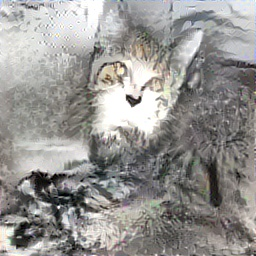
\includegraphics[width=\textwidth]{figure/baseline3/chinese.jpg}
    \caption{Chinese painting}
    \label{fig::base35}
  \end{subfigure}
  %	\vspace{-1mm}
  \caption{Baseline 3: Smoothing, Canny, DIS, and feeding AWAST with the detailed image}
  \label{fig::cannyplus}
  %
  \begin{subfigure}[b]{0.18\textwidth}
    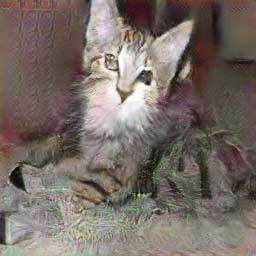
\includegraphics[width=\textwidth]{figure/baseline1/pix2pix.jpg}
    \caption{Detailed Image}
    \label{fig::base41}
  \end{subfigure}
  ~
  %
  \begin{subfigure}[b]{0.18\textwidth}
    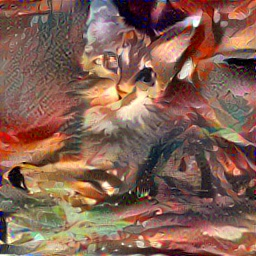
\includegraphics[width=\textwidth]{figure/baseline1/yys.jpg}
    \caption{Onmyoji}
    \label{fig::base42}
  \end{subfigure}
  %
  \begin{subfigure}[b]{0.18\textwidth}
    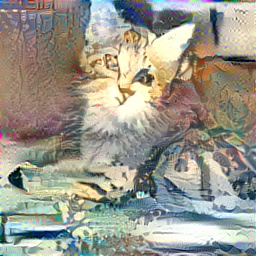
\includegraphics[width=\textwidth]{figure/baseline1/fsh.jpg}
    \caption{Ukiyo-e}
    \label{fig::base43}
  \end{subfigure}
  %
  \begin{subfigure}[b]{0.18\textwidth}
    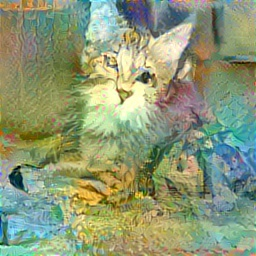
\includegraphics[width=\textwidth]{figure/baseline1/fg.jpg}
  \caption{Van Gogh}
    \label{fig::base44}
  \end{subfigure}
  %
  \begin{subfigure}[b]{0.18\textwidth}
    \includegraphics[width=\textwidth]{figure/baseline1/chinese.jpg}
    \caption{Chinese painting}
    \label{fig::base45}
  \end{subfigure}
  %	\vspace{-1mm}
  \caption{Our scheme: Smoothing, extracting of pencil sketch, DIS, and feeding AWAST with the detailed image}
  \label{fig::sketchplus}
\end{figure*}

\subsection{Baselines and Analysis}

\subsubsection{Baselines}
We set some baselines to show our method of assembling the model works best:

\textbf{Baseline 1:} Shown in Fig.\ref{fig::cannyonly}: reality image $\rightarrow$ Canny image $\rightarrow$ style image.

\textbf{Baseline 2:} Shown in Fig.\ref{fig::sketchonly}: reality image $\rightarrow$ smoothing image $\rightarrow$ sketch image $\rightarrow$ style image.

\textbf{Baseline 3:} Shown in Fig.\ref{fig::cannyplus}: reality image $\rightarrow$ smoothing image $\rightarrow$ Canny image $\rightarrow$ detailed image $\rightarrow$ style image.

\textbf{Our scheme:} In Fig.\ref{fig::sketchplus}: reality image $\rightarrow$ smoothing image $\rightarrow$ pencil sketch $\rightarrow$ detailed image $\rightarrow$ style image.

\subsubsection{Analysis of baselines}
As shown in Fig.\ref{fig::cannyonly}, the synthesized stylized image is quite blurring. There are many noisy points that can't converge to the optimizing object. And the features of the content are not extracted successfully. So there are some areas just copy the pattern of the style samples. For example, in Fig.\ref{fig::base13}, near the cat's feet, the pattern is just like the tide which comes from the style samples of Ukiyo-e style. This is because the information in the edge picture is not enough to push the AWAST synthesize the objetive result, so as to people's freehand sketch. So, the information generating process, DIS, is needed.

In Fig.\ref{fig::sketchonly}, we can see that by smoothing and pencil sketch extraction, the results are much better. The problems of pattern copying like Baseline $1$ are improved and the shape of the cat looks more clear. At the same time, the style image is not so blurring as Baseline $1$. These improvements suggest that the smoothing and pencil sketch extraction are quite helpful to extract the key information in the reality image while weak the noise. By comparing Fig.\ref{fig::base11} and Fig.\ref{fig::base21}, the sketch in Baseline $2$ is more like human freehand sketch on the continuity and directions.

Fig.\ref{fig::cannyplus} represents the final results of Baseline $3$, which includes smoothing, canny, DIS, and AWAST. Compared to Baseline $1$, the results are much more beautiful. The shape of the cat is more clear and the problem of pattern copying is solved. The shade of the styles is also more natural. The details are also more clear. In Fig.\ref{fig::base35}, for example, the eyes of the cat become yellow which is different from the color of its body. This means the detail of the cat's eyes is noticed and emphasize by the AWAST model.

Our final scheme is shown in Fig.\ref{fig::sketchplus}, including smoothing, pencil sketch extraction, DIS, and AWAST. The performance improves a lot comparing to Baseline $3$.
For example, in Fig.\ref{fig::base45}, eyes of the cat are much more vivid and the patterns of fur and beard on its head and body are detailed.
\begin{figure*}[!h]
  \centering
  \begin{subfigure}[b]{0.33\textwidth}
    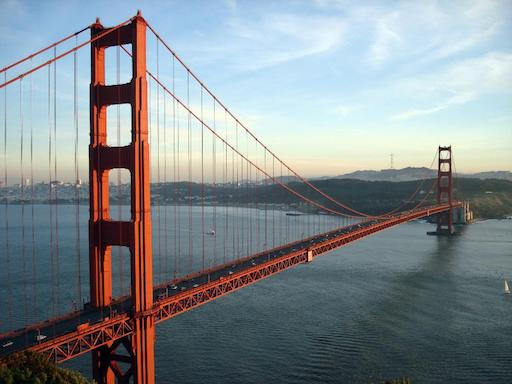
\includegraphics[width=\textwidth]{figure/contentgoldbridge.jpg}
    \caption{Reality (Golden Gate Bridge)}
    \label{fig::goldreal}
  \end{subfigure}
  %
  \begin{subfigure}[b]{0.33\textwidth}
    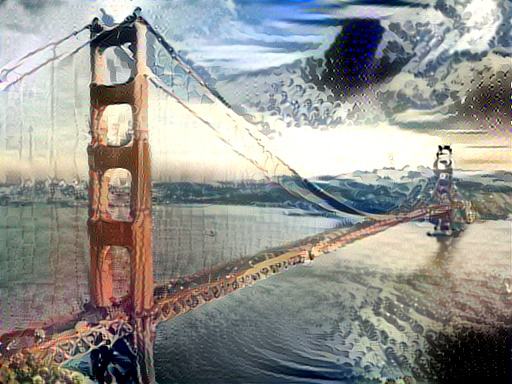
\includegraphics[width=\textwidth]{figure/stdgoldbridge.jpg}
    \caption{Result of Gatys et al.}
    \label{fig::goldgatys}
  \end{subfigure}
  %
  \begin{subfigure}[b]{0.33\textwidth}
    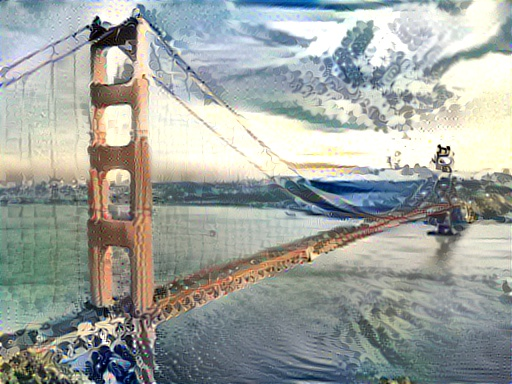
\includegraphics[width=\textwidth]{figure/ourgoldbridge.jpg}
    \caption{Result of Ours}
    \label{fig::goldours}
  \end{subfigure}
  \caption{Performance analysis of AWAST}
  \label{fig::goldbridge}
\end{figure*}

\begin{figure*}[!h]
\begin{subfigure}[b]{0.16\textwidth}
  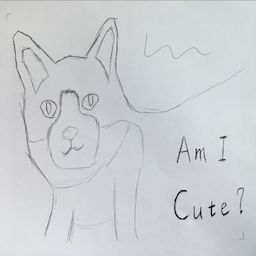
\includegraphics[width=\textwidth]{figure/realdraw/src.jpg}
  \caption{Freehand sketch}
  \label{fig::freehand}
\end{subfigure}
%
\begin{subfigure}[b]{0.16\textwidth}
  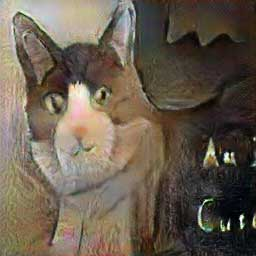
\includegraphics[width=\textwidth]{figure/realdraw/pix2pix.jpg}
  \caption{Detailed image}
  \label{fig::realdetailed}
\end{subfigure}
%
\begin{subfigure}[b]{0.16\textwidth}
  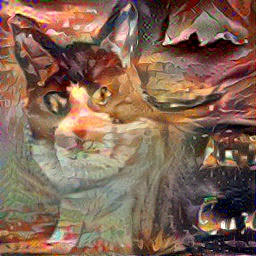
\includegraphics[width=\textwidth]{figure/realdraw/yys.jpg}
  \caption{Onmyoji}
  \label{fig::realyys}
\end{subfigure}
%
\begin{subfigure}[b]{0.16\textwidth}
  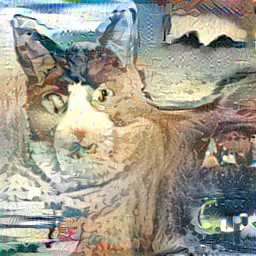
\includegraphics[width=\textwidth]{figure/realdraw/fsh.jpg}
  \caption{Ukiyo-e}
  \label{fig::reslfsh}
\end{subfigure}
%
\begin{subfigure}[b]{0.16\textwidth}
  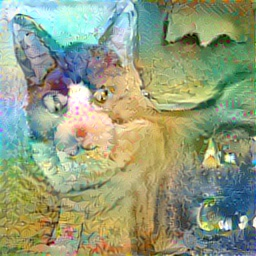
\includegraphics[width=\textwidth]{figure/realdraw/fg.jpg}
\caption{Van Gogh}
  \label{fig::realfg}
\end{subfigure}
%
\begin{subfigure}[b]{0.16\textwidth}
  \includegraphics[width=\textwidth]{figure/realdraw/chinese.jpg}
  \caption{Chinese painting}
  \label{fig::realchinese}
\end{subfigure}
%	\vspace{-1mm}
\caption{Test result of real freehand sketch of cat}
\label{fig::realtest}
\end{figure*}

\FloatBarrier
On Fig.\ref{fig::base42}, the style transfer is active and does not break the shape of the cat while on Fig.\ref{fig::base32}, the style mix the cat's body and the environment.

\begin{figure}
    \includegraphics[width=0.48\textwidth]{figure/fshstyle.pdf}
    \caption{Images of Ukiyo-e style to analyze AWAST}
    \label{fig::fshstyle}
\end{figure}

\subsubsection{Analysis of AWAST}
We use $6$ images in Fig~\ref{fig::fshstyle} of Ukiyo-e style to analyze the performance of AWAST. However, one image of them is coverd by black color. The experiment result when iterations $iter=2500$ is shown in Fig.\ref{fig::goldbridge}. The result of Gatys et al. in Fig.\ref{fig::goldgatys} appears to have many black areas, which is attributed to taking the patterns of black. This is because the blending method of them is simply taking the average of multiple features. Our method in Fig.\ref{fig::goldours} is steadier and more natural, because ASW based on PageRank algorithm weaks the weight of the unusual styles like black images and emphasizes the right styles in the other $5$ images.

\subsection{Test}
For convenience, all the experiment above is based on the test set which is generated by SIE model. However, our goal is to transform a real freehand sketch to an artistic painting. So we take an $A4$ paper and a pencil and draw a cat sketch by hand, which is shown in Fig.\ref{fig::freehand}. This is quite easy actually. We simply take a photo with our mobile-phone and then feed it into the DIS and the AWAST model. To make the result compared fairly, we still use the same style samples. the result is shown in Fig.\ref{fig::realtest}.

\section{Conclusions}
To be an artist is always many people's dream. In this paper, we propose \textsc{Line Artist} to synthesize appealing paintings with freehand sketch. To achieve this goal, we propose the SIE model to smooth the images and extract the sketch to build new datasets. The DIS model based on GAN allow the sketch drew by users to generate more details and looks natural. The AWAST model propose an novel algorithm based on PageRank to adaptively combining styles from multiple painting samples. Our results are prove to be vivid, artistic, and adapted to different styles stably. There are also some issues need to be improved. In the DIS and the AWAST model, the synthesis is not real-time. However, \textsc{Line Artist} still has the potential to become an powerful entertainment APP and assistant of artists.


\newpage

{\small
\bibliographystyle{ieee}
\bibliography{egbib}
}

\end{document}
